\chapter{提案手法の実装とシミュレーションの環境}
\label{chap:implementation_and_experimentation}

\section{Omnet++とDTNsimを用いた評価環境}
Omnet++はネットワークシミュレータの構築を目的としたオープンソースのプラットフォームであり, 
既存の通信プロトコルや物理層のシミュレーションを実装しているほか, 
各ノードにC++でのアプリケーションを実装し拡張することが可能である. 
DTNsimはOmnet++のフレームワーク上で動作するDTNのシミュレーターであり, 
ION-DTN, HDTNなどの種々のDTN実装が動作するネットワークをシミュレートすることができ, 
各種CGRのバリエーションにも対応する. そのため本研究ではこのOmnet++とDTNsimを用いて
宇宙で運用されているDTNをシミュレーションを行う. 

\section{2030・2040年代のDTNを想定したシナリオとパラメータ}
本実験においては, 2030年代に地球・月間, 2040年代に地球・月・火星間にまたがるDTNを運用していることを想定し, 
そのうち任意の2天体間について既存手法と本研究の提案手法の実装とシミュレーションを行い, 
本研究の提案の有効性について検証する. そのため任意の2天体間のDTNネットワークとして, 
図\ref{fig:experimentation_topology}のようなトポロジーを想定する. 
ノード1から3は天体A, ノード4から6はそれぞれ天体Bに属するDTNノードであり, 
ノード1と6はそれぞれの地表DTNのノード, ノード2から5はそれぞれの天体の軌道上にある
宇宙のDTNノードである. 
\ref{section:2030年代の地球・月間を想定したトポロジー}項では
2030年代の地球・月間のDTNにおけるシナリオ, 
\ref{section:2040年代の地球・月・火星間を想定したトポロジー}項では
2040年代の地球・月・火星間のDTNにおけるシナリオを説明する. 
\begin{figure}[tbh]
    \centering
    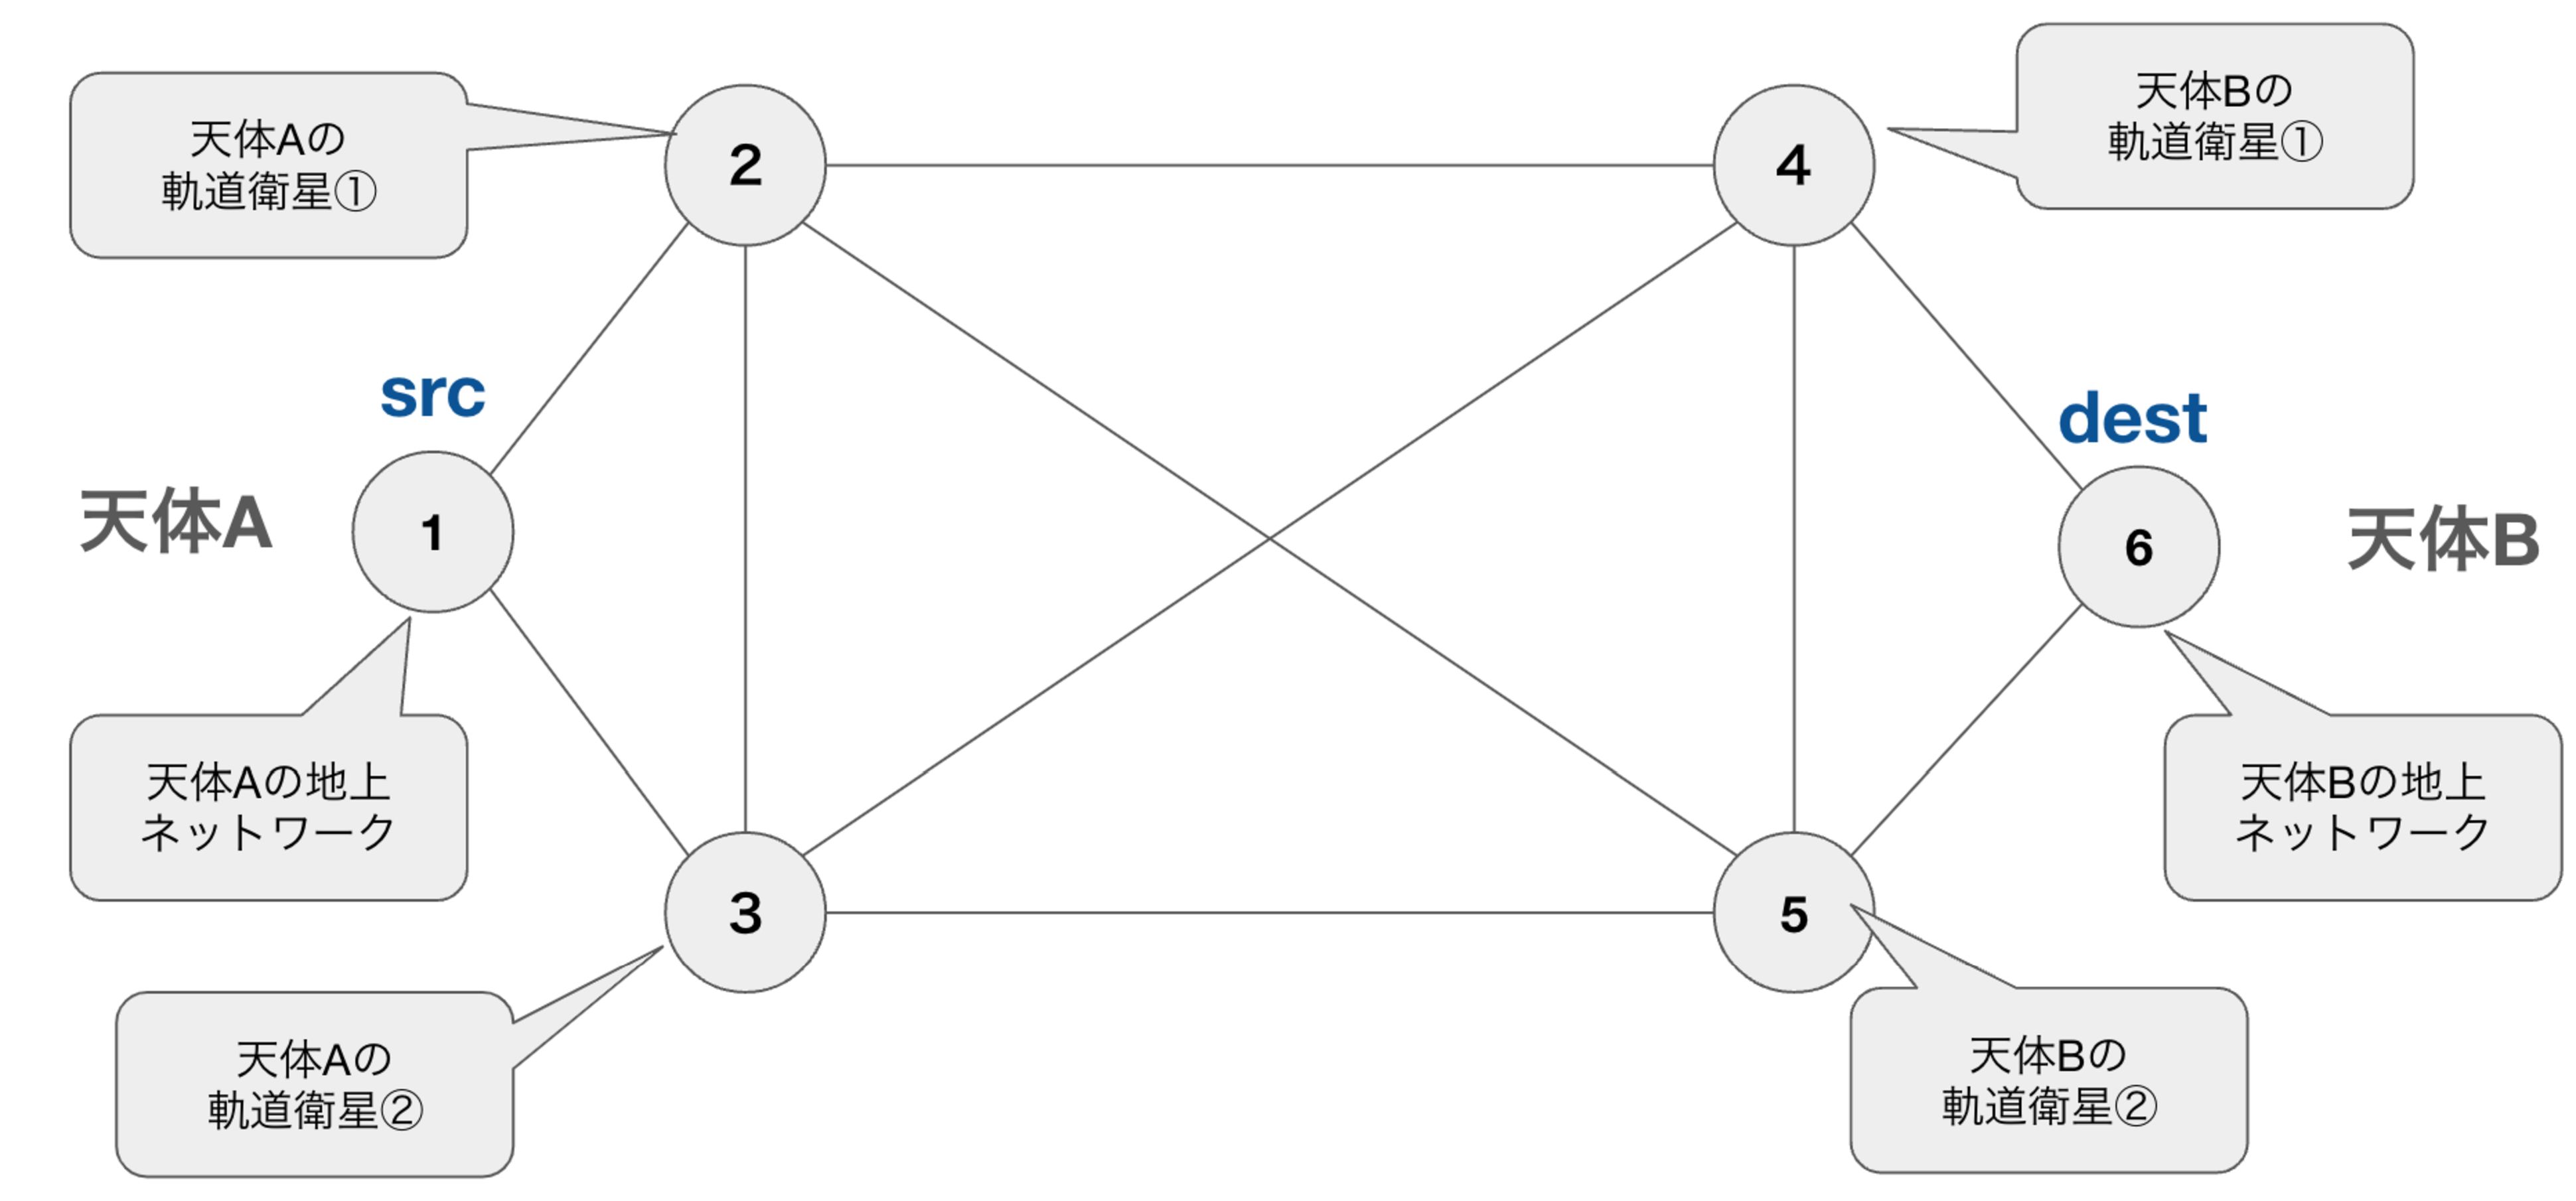
\includegraphics[width=0.7\textheight]{img/thesis_Sample_topology.pdf}
    \caption{本実験で用いるトポロジー}
    \label{fig:experimentation_topology}
    \begin{minipage}{\textwidth}
        \raggedright
        \vspace{3mm}
        ノード1は天体Aの地上DTNネットワークを代表したノード, ノード2とノード3は
        天体Aの軌道上に存在する宇宙のDTNノード, ノード4とノード5は
        天体Bの軌道上に存在する宇宙のDTNノード, 
        ノード6は天体Bの地上DTNネットワークを代表したノードを示す. 
    \end{minipage}
\end{figure}

\subsection{2030年代の地球・月間を想定したトポロジー}
\label{section:2030年代の地球・月間を想定したトポロジー}
2030年代の人類の月における活動区域は当面月の南極域になることが予想され, 
図\ref{fig:artemis_moon_station_orbit}に示すように, 
月南極域との通信可能時間の長いNRHO軌道の利用が検討されている. 
本実験ではこのNRHO軌道を利用した地球・月間のDTNネットワークを想定し, 
図\ref{fig:experimentation_topology}のトポロジーにおいて, 
それぞれ以下の構成を用いる. 
\begin{itemize}
    \item 天体A: 地球
    \item 天体B: 月
    \item ノード1: 地球の地上DTNノード
    \item ノード2: 地球の静止軌道上に存在するDTNノード
    \item ノード3: 地球の静止軌道上に存在するDTNノード
    \item ノード4: 月のNRHO軌道上に存在するDTNノード
    \item ノード5: 月のNRHO軌道上に存在するDTNノード
    \item ノード6: 月の地表DTNノード
\end{itemize}
地球の静止軌道上に存在するDTNノードは地球に対してほぼ円軌道を描き, 地表からおよそ36,000kmの高度を飛行する. 
また月のNRHO軌道上に存在するDTNノードは,  月面から4,000km$\sim$75,000km程度を極端な楕円軌道を描いて飛行する. 
この時地球の静止軌道上に存在するDTNノードと月のNRHO軌道上に存在するDTNノードの距離は308,000km$\sim$415,000km程度になる. 
これらを考慮し, ノード間の距離は以下のように設定した. 
\begin{itemize}
    \item ノード1 - ノード2またはノード3 間: 0.12光秒
    \item ノード2 - ノード3 間: 0.12光秒
    \item ノード2またはノード3 - ノード4またはノード5  間: 1.03光秒$\sim$1.38光秒
    \item ノード4 - ノード5  間: 0.12光秒
    \item ノード4またはノード5 - ノード6  間: 0.13光秒
\end{itemize}

\subsection{2040年代の地球・月・火星間を想定したトポロジー}
\label{section:2040年代の地球・月・火星間を想定したトポロジー}
2040年代には活動区域は火星にまで広がっていることが予想される. 
本実験では\ref{section:2030年代の地球・月間を想定したトポロジー}項で
述べた地球・月間のDTNネットワークと同様, 以下の構成を用いる. 
\begin{itemize}
    \item 天体A: 地球
    \item 天体B: 火星
    \item ノード1: 地球の地上DTNノード
    \item ノード2: 地球の静止軌道上に存在するDTNノード
    \item ノード3: 地球の静止軌道上に存在するDTNノード
    \item ノード4: 火星の軌道上に存在するDTNノード
    \item ノード5: 火星の軌道上に存在するDTNノード
    \item ノード6: 火星の地表DTNノード
\end{itemize}
火星における運用は現時点では未定ではあるものの, 
火星の開発初期においてはおおよそ月における運用と同様のものになると考えられる. 
そのためノード間の距離は以下のように設定した. 
\begin{itemize}
    \item ノード1 - ノード2またはノード3 間: 0.12光秒
    \item ノード2 - ノード3 間: 0.12光秒
    \item ノード2またはノード3 - ノード4またはノード5  間: 480光秒$\sim$1200光秒
    \item ノード4 - ノード5  間: 0.12光秒
    \item ノード4またはノード5 - ノード6  間: 0.13光秒
\end{itemize}

\subsection{シミュレーションで用いるバンドルトラフィック}
\label{section:シミュレーションで用いるバンドルトラフィック}
本実験では図\ref{fig:experimentation_topology}のトポロジーにおいて, 
ノード1からノード6に向かう, すなわち天体Aの地上DTNネットワークから天体Bの地上DTNネットワークに
向けてのトラフィックを想定する. DTNsimではトラフィックとして生成するバンドルについて様々な
パラメータを設定することが可能である. 以下に例を上げる. 
\begin{itemize}
    \item シミュレーション全体におけるバンドルの総生成数(bundlesNumber)
    \item 生成したバンドルの送信元ノードのendpoint ID(sourceEid)
    \item 生成したバンドルの宛先ノードのendpoint ID(destinationEid)
    \item バンドル生成イベントごとのバンドルのサイズ(bytes)(size)
    \item バンドル生成イベントの間隔(秒)(interval)
\end{itemize}
実際の宇宙インターネットにおけるトラフィックの発生状況は当然時刻変動するものであるが, 
本論文におけるシミュレーションでは単位時間あたりのトラフィック量は概ね一定であると仮定した. 
また天体Aの地上DTNネットワークから天体Bの地上DTNネットワークに向けたトラフィックを想定し, 
図\ref{fig:experimentation_topology}のトポロジーにおいて, ノード1からノード6に向かうトラフィックを
生成する. そのため, 本論文におけるシミュレーションでは上記のパラメータに対してそれぞれ以下の値を用いた. 
\begin{itemize}
    \item bundlesNumber: 1800
    \item sourceEid: 1
    \item destinationEid: 6
    \item size: 1500
    \item interval: 1
\end{itemize}
